\section{Microarchitecture}
\label{sec:arch}

\subsection{Residue and metadata-augmented variants}
\label{sec:arch-variants}

\fpfourres{} adds a second activation block $\mathit{ar}$ with its own scale
$s_{ar}=2^{S_{ar}-127}$, quantising the residual of the primary block against
plain \fpfour{} weights. The dot product carries two independent scales,
%
\begin{equation}
  \label{eq:res-base}
  \mathit{acc}' = s_a s_w \sum_i a_i w_i
                + s_{ar} s_w \sum_i \mathit{ar}_i w_i + \mathit{acc},
\end{equation}
%
which factors on the primary scale as
%
\begin{equation}
  \label{eq:res-factor}
  \mathit{acc}' = s_a s_w\!\left( \sum_i a_i w_i
                  + \frac{s_{ar}}{s_a} \sum_i \mathit{ar}_i w_i
                  + \frac{\mathit{acc}}{s_a s_w} \right).
\end{equation}
%
The ratio $s_{ar}/s_a = 2^{S_{ar}-S_a}$ is again a shift, by
$\delta = S_a - S_{ar} \ge 0$; \S\ref{sec:arch-residue} establishes the
non-negativity and its role in placement. The primary product term reuses the
\fpfour{} datapath unchanged.

\mtwo{}~\cite{m2xfp2026} retains E2M1 elements and adds per-instruction
metadata. Within each 8-element subgroup, two bits extend the largest-magnitude
activation element to E2M3, and two bits refine the weight subgroup scale to
$(1+\kappa/4)\,2^{S}$, $\kappa\in\{0,1,2,3\}$. The scaled sum of products
becomes
%
\begin{equation}
  \label{eq:m2}
  \mathit{acc}' = s_a s_w \sum_g \left(1+\tfrac{\kappa_g}{4}\right)
                  \sum_{i \in g} a_i w_i + \mathit{acc},
\end{equation}
%
in which $a_i$ denotes the top-1 element's E2M3-corrected value for the
subgroup's single largest-magnitude activation and its plain E2M1 value
otherwise, and the $\kappa_g$ factor is a per-subgroup shift-and-add on the
partial sum, not a multiplication.

\subsection{Instruction interface}
\label{sec:arch-isa}

Instructions reuse the R4-type FMADD.S operand layout, so a third source needs
no host register-file change.

% Merged instruction set + operand map. R4-type custom-0 opcode 0x0B; funct2
% selects the MX format, funct3 the operation. Only MXFP4R takes two native
% instructions (stated in the caption; no separate Insns/dp column needed).
% Column headers abbreviated (f3/f2, Elems) with symbol-footnote expansions
% to fit the operand columns in the same single-column float; symbol
% definitions and dual-read/32-bit-read facts follow below.
\begin{table}[t]
  \centering
  \caption{Instruction set and operand map. R4-type, custom-0 opcode
           \insn{0x0B}; \insn{funct2} selects the MX format, \insn{funct3}
           the operation. \fpfourres{} requires two native instructions,
           since it carries a third \SI{64}{\bit} source
           and a second block scale (\S\ref{sec:arch-residue}).}
  \label{tab:isa}
  \scriptsize
  \setlength{\tabcolsep}{2.3pt}
  \renewcommand{\arraystretch}{1.15}
  \resizebox{\columnwidth}{!}{%
  \begin{tabular}{|l|l|c|c|c|c|c|}
    \hline
    Format & Mnemonic & \insn{f3/f2}\rlap{$^{\ast}$} &
      Elems\rlap{$^{\dagger}$} &
      \insn{rs1} & \insn{rs2} & \insn{rs3} \\
    \hline
    \fpfour  & \MXFUSED & 011/00 & 16
        & $p_A$ & $p_W$ & $\{x_W,x_A,\mathit{acc}\}$ \\
    \hline
    \fpeight & \MXFUSED & 011/11 &  8
        & $p_A$ & $p_W$ & $\{x_W,x_A,\mathit{acc}\}$ \\
    \hline
    \mtwo    & \MXFUSED & 011/10 & 16
        & $p_A$ & $p_W$ & $\{\mathrm{md},x_W,x_A,\mathit{acc}\}$ \\
    \hline
    \multirow{2}{*}{\fpfourres}
             & \MXDOTP  & 000/01 & 16
                 & $p_A$ & $p_W$ & $p_{Ar}$ \\
    \cline{2-7}
             & \MXFINAL & 001/01 & ---
                 & $\{x_A,x_{Ar},x_W\}$ & $\mathit{acc}$ & --- \\
    \hline
  \end{tabular}%
  }
  \\[2pt]
  \begin{minipage}{\columnwidth}
    \scriptsize
    \textsuperscript{*}\insn{funct3}/\insn{funct2}.
    \textsuperscript{\textdagger}Elements per instruction.
    $p_A,p_W,p_{Ar}$: packed activation/weight/residue-activation vectors;
    $x_A,x_{Ar},x_W$: E8M0 block scales; \textit{acc}: FP32 accumulator;
    braces denote fields packed into one register word. $p_A,p_W,p_{Ar}$ and
    \MXFUSED's \insn{rs3} are \SI{64}{\bit} dual-read register pairs;
    \MXFINAL's \insn{rs1},\insn{rs2} are plain \SI{32}{\bit} reads.
    \MXDOTP{} writes no register; \MXFINAL{} and \MXFUSED{} write the FP32
    result.
  \end{minipage}
\end{table}

\MXFUSED{} is a single-instruction operation for \fpfour, \fpeight, and \mtwo.
\fpfourres{} instead needs three genuine 64-bit sources and two independent
block scales at once, which exceeds a three-read-port register file, so it is
issued as the \MXDOTP/\MXFINAL{} pair (\S\ref{sec:arch-residue}). For \mtwo{},
operand order is significant: \insn{rs1} carries activations and \insn{rs2}
weights.

\subsection{Scale-free accumulation frame}
\label{sec:arch-frame}

Every engine realises~\eqref{eq:factor} through a fixed-point frame in which
the sum of products is resident and the accumulator, rather than the products,
absorbs the block scale~\cite{lutz2024fp8dot,islamoglu2025mxdotp}. The sum of
products occupies a format-specific anchor position, where frame bit $b$ carries
weight $2^{b-\alpha}$ and the anchor $\alpha$ is chosen so that the smallest
representable quantum aligns with bit~0; every product is then frame-resident
without a shifter. The anchor thus tracks each format's smallest quantum:
$\alpha=2$ for \fpfour's E2M1 products, $32$ for \fpeight, whose smallest E5M2
subnormal product is $2^{-32}$,\footnote{The reference
implementation~\cite{islamoglu2025mxdotp} anchors at $34$; its per-element decode
pads the E5M2 mantissa by one bit, shifting the same 95-bit frame up two
positions, so the two are value-identical.} and $6$ for \mtwo, set by the $1/64$
quantum its $(1+\kappa/4)$ refinement introduces; \fpfourres{} shares \fpfour's
anchor. The FP32 accumulator enters by a shift of
$E_{\mathit{acc}} - C_\alpha - (S_a{+}S_b{-}254)$, where $C_\alpha = 150-\alpha$
is a compile-time constant, and bits below the frame are retained in a
$\mathrm{REMAIN}$-bit extension with a sticky bit. The scale contributes only to
the final exponent.

The consequence is that frame width is a function of the element format alone
and is independent of the E8M0 scale range, so each engine is exact to
round-to-nearest-even over every legal scale pair and every FP32 accumulator at
a width set by its own format. Applying the scheme across four formats requires
a distinct frame geometry for each; the constants are derived in closed form and
listed in Table~\ref{tab:frames}.

\begin{table}[t]
  \centering
  \caption{Derived sliding-frame constants. Frame width is set by the element
           format alone; the E8M0 scale range does not appear.}
  \label{tab:frames}
  \setlength{\tabcolsep}{4pt}
  \renewcommand{\arraystretch}{1.15}
  \begin{tabular}{|l|c|c|c|c|c|}
    \hline
    Engine & Anchor $\anchor$ & $\Sigma_{\mathrm{P}}$\rlap{$^{\ast}$} & Frame & REMAIN & LZC \\
           &                  & (bits)                & (bits) & (bits) & (bits) \\
    \hline
    \fpfour     &  2 & 12 & 38 & 25 &  63 \\
    \hline
    \fpeight    & 32 & 69 & 95 & 25 & 120 \\
    \hline
    \mtwo       &  6 & 17 & 43 & 25 &  68 \\
    \hline
    \fpfourres  &  2 & 12\rlap{$^{\dagger}$} & 38 & 36 &  74 \\
    \hline
  \end{tabular}
  \\[2pt]
  \begin{minipage}{\columnwidth}
    \footnotesize
    $^{\ast}$Unsigned sum-of-products field resident in the frame word.
    $^{\dagger}$Two product terms at independent scales
    (\S\ref{sec:arch-residue}); the wider REMAIN follows from cancellation
    between them rather than against the accumulator.
  \end{minipage}
\end{table}

Three of the table's columns are linked as consistency checks: Frame $=
26+\Sigma_{\mathrm{P}}$ (sign, 24-bit accumulator mantissa, guard bit, and the
$\Sigma_{\mathrm{P}}$ field) and $\text{LZC}=\text{Frame}+\mathrm{REMAIN}$
(the leading-zero counter spans the full pre-normalisation word, not the frame
alone); both hold in every row.

Two of the derived bounds are non-obvious. The $\mathrm{REMAIN}$ extension must
guarantee that, under catastrophic cancellation with the sticky bit asserted,
the surviving leading one cannot fall below the round-bit position; this bound
depends only on the 24-bit accumulator mantissa, not on anchor or
sum-of-products width, giving $\mathrm{REMAIN}=25$ identically for \fpfour,
\fpeight, and \mtwo, with the two-product residue frame widening it
(\S\ref{sec:arch-residue}). Consequently, no wider extension is required,
avoiding unnecessary leading-zero detection width. Frame width follows a
similar no-overflow argument bounding the accumulator against the resident sum
of products, so no in-frame saturation logic is instantiated in any engine.

\begin{figure}[t]
  \centering
  \resizebox{\columnwidth}{!}{% Fig. 1 -- per-format scale-free accumulation frame, to scale, aligned at bit 0.
% Each field's LEFT edge is computed directly (cumulative offset from bit 0)
% rather than chained off a neighbour's anchor, so fields cannot overlap.
\begin{tikzpicture}[
  font=\scriptsize,
  seg/.style={draw, minimum height=5.4mm, inner sep=0pt, outer sep=0pt, anchor=south west},
  tny/.style={font=\tiny},
]
  \def\u{0.052}\def\ob{0.16}\def\ha{0.56}\def\lx{-5.55}
  \def\wA{24*\u}  % 24-bit acc mantissa field width (constant across formats)

  % {y}{key}{disp}{SoP bits}{REMAIN bits}{annotate top row 0/1}
  \newcommand{\frmrow}[6]{%
    \pgfmathsetmacro{\wS}{#4*\u}\pgfmathsetmacro{\wR}{#5*\u}%
    \pgfmathsetmacro{\wAv}{\wA}%
    % left edges, computed directly from bit 0 (x=0), never chained off a
    % neighbour's opposite corner -- this is what the overlap bug violated.
    \pgfmathsetmacro{\xSoP}{-\wS}%
    \pgfmathsetmacro{\xG}{\xSoP-\ob}%
    \pgfmathsetmacro{\xAcc}{\xG-\wAv}%
    \pgfmathsetmacro{\xSgn}{\xAcc-\ob}%
    \node[seg, fill=black!8,   minimum width=\ob cm] (s#2)   at (\xSgn,#1) {};
    \node[seg, fill=orange!24, minimum width=\wAv cm] (acc#2) at (\xAcc,#1) {\tiny 24};
    \node[seg, fill=black!8,   minimum width=\ob cm] (g#2)   at (\xG,#1)   {};
    \node[seg, fill=blue!16,   minimum width=\wS cm] (sop#2) at (\xSoP,#1) {\tiny #4};
    \node[seg, fill=black!12,  minimum width=\wR cm] (rem#2) at (0,#1)     {\tiny #5};
    \node[seg, fill=black!8,   minimum width=\ob cm] (st#2)  at ($(rem#2.south east)$) {};
    \draw[very thick] (0,#1) -- (0,{#1+\ha});
    \node[anchor=east] at (\lx,{#1+\ha/2}) {#3};
    \ifnum#6=1
      \node[tny, anchor=south] at ($(acc#2.north)+(0,0.58)$) {accumulator slides};
      \draw[-{Stealth[length=3pt]}, thick]
           ($(acc#2.north west)+(0.10,0.40)$) -- ($(acc#2.north east)+(-0.10,0.40)$);
      \node[tny, anchor=south] at ($(sop#2.north)+(0,0.16)$) {$\sum a_ib_i$ resident (no shifter)};
      \node[tny, anchor=south] at (0,{#1+\ha+0.08}) {bit\,0};
      \draw[decorate, decoration={brace, amplitude=3pt}]
           ($(rem#2.south east)+(0,-0.06)$)
           -- node[below, tny, yshift=1pt] {leading-one scan (LZC)}
           ($(s#2.south east)+(0,-0.06)$);
    \fi
  }

  \frmrow{0.0}{FF}{MXFP8}{69}{25}{1}
  \frmrow{-1.25}{MM}{M$^2$XFP4}{17}{25}{0}
  \frmrow{-2.20}{RR}{MXFP4R}{12}{36}{0}
  \frmrow{-3.15}{PP}{MXFP4}{12}{25}{0}

  % ---- block scale bypasses the wide word, enters the exponent only ----
  \coordinate (base) at (\lx,{-3.15-0.55});
  \node[tny, anchor=west, align=center] (bscale) at ($(base)+(0.55,-0.30)$)
       {block scale\\$S_a{+}S_b$};
  \node[draw, dashed, rounded corners, fill=green!8, tny, anchor=west]
       (rexp) at ($(bscale.east)+(0.55,0)$) {result exponent};
  \draw[-{Stealth[length=4pt]}, dashed, green!45!black] (bscale.east) -- (rexp.west);
  \node[tny, anchor=west] at ($(rexp.east)+(0.12,0)$)
       {applied here only --- never the wide word};

  % ---- field legend ----
  \node[tny, anchor=west, align=left] at ($(base)+(0.55,-0.86)$)
       {\tikz\draw[fill=orange!24](0,0)rectangle(0.22,0.16);\, 24\,b acc mantissa (slides)\quad
        \tikz\draw[fill=blue!16](0,0)rectangle(0.22,0.16);\, sum of products ($\Sigma P$)\quad
        \tikz\draw[fill=black!12](0,0)rectangle(0.22,0.16);\, REMAIN\,$+$\,sticky};
\end{tikzpicture}}
\caption{Per-format scale-free accumulation frame, drawn to scale and aligned
  at bit~0. The sum of products is resident and exact at each format's anchor;
  only the FP32 accumulator slides (Table~\ref{tab:frames} lists all widths).}
  \label{fig:frame}
\end{figure}

\subsection{Format-specialised engines}
\label{sec:arch-engines}

Each format is realised as an independent engine instantiating the frame at its
own constants. Width-parameterised blocks---leading-zero count,
normalise-and-round, and the accumulator slide---are shared as modules
elaborated at each format's width, so \fpfour{} instantiates a 63-bit
leading-zero count where \fpeight{} instantiates a 120-bit one. The front-end
decode, multiply array, and reduction tree are not shared, as these are
format-specific: a single \fpeight{} engine's decode covers both E4M3 and E5M2
elements, and unifying \mtwo's widened top-1 lane (\S\ref{sec:arch-m2}) with
\fpfour's narrower lanes into one common array would impose the wider format's
cost on the narrower one. Preserving per-format module instances also allows
area and timing to be attributed per format
(\S\ref{sec:eval}).

Each fused engine is a five-stage pipeline---input capture, front-end output,
frame word, leading-one result, and result register---with a single global
stall that freezes all stages when the result register is occupied and the
consumer is not ready. Each stage carries an independent valid bit and
instruction-identifier sideband, so the three fused-format engines accept one
instruction per cycle and the interface layer restores program order through an
order queue.

\begin{figure}[t]
  \centering
  \resizebox{\columnwidth}{!}{% Fig. 2 -- MXFP4 fused-engine datapath (exemplar of the four format-specialised
% engines). Arithmetic drawn as circles (x=multiply, +=add), control/scan stages
% as boxes, matching mxdotp_fused_engine.sv / mx_acc_slide / mx_find_lead /
% mx_finalize exactly (widths verified against the RTL ports).
\begin{tikzpicture}[
  font=\small, >=Stealth,
  mul/.style={circle, draw, minimum size=6.5mm, inner sep=0pt, fill=blue!6},
  add/.style={circle, draw, minimum size=6.5mm, inner sep=0pt, fill=orange!10},
  shiftbox/.style={diamond, draw, aspect=2.4, minimum width=15mm, minimum height=8mm,
                   inner sep=0pt, fill=violet!8},
  stg/.style={draw, rounded corners=1pt, align=center, minimum height=9mm,
              minimum width=17mm, fill=blue!7, font=\small},
  opnd/.style={draw, rounded corners=1pt, align=center, minimum height=7mm,
               font=\small, fill=black!4},
  lbl/.style={font=\scriptsize, align=center},
  fl/.style={-{Stealth[length=5pt]}},
  scl/.style={-{Stealth[length=5pt]}, green!40!black, thick},
]
  %=================== operand row ===================
  \node[opnd, minimum width=17mm] (rs1) at (0,5.0)   {\texttt{rs1}$=A$\\16$\times$E2M1};
  \node[opnd, minimum width=17mm] (rs2) at (3.0,5.0) {\texttt{rs2}$=B$\\16$\times$E2M1};
  \node[opnd, minimum width=26mm] (rs3) at (10.0,5.0) {\texttt{rs3}: $S_a,S_b$ (8\,b ea.), old acc (FP32)};

  %=================== 16-lane multiply-accumulate ===================
  \node[mul] (m0) at (0.4,3.6) {$\otimes$};
  \node[mul] (m1) at (1.6,3.2) {$\otimes$};
  \node[lbl] at (2.35,3.05) {$\cdots$};
  \node[mul] (m15) at (3.1,3.6) {$\otimes$};
  \node[lbl, anchor=north] at (m0.south)  {\shortstack{$a_0$\\$b_0$}};
  \node[lbl, anchor=north] at (m1.south)  {\shortstack{$a_1$\\$b_1$}};
  \node[lbl, anchor=north] at (m15.south) {\shortstack{$a_{15}$\\$b_{15}$}};
  \draw[fl] (rs1) -- (1.4,4.4) -- (m1.north);
  \draw[fl] (rs2) -- (1.6,4.4) -- (m1.north);

  \node[isosceles triangle, draw, shape border rotate=-90, isosceles triangle apex angle=60,
        minimum height=16mm, fill=orange!8] (sumtri) at (5.0,3.6) {};
  \node[lbl] at ($(sumtri.center)+(-0.05,0)$) {$\Sigma$};
  \draw[fl] (m0)  -- ($(sumtri.west)+(0,0.55)$);
  \draw[fl] (m1)  -- (sumtri.west);
  \draw[fl] (m15) -- ($(sumtri.west)+(0,-0.55)$);
  \node[lbl] at (1.85,3.9) {9\,b product};

  \node[stg, minimum width=16mm, fill=blue!14] (sop) at (7.1,3.6) {SoP\\13\,b, $\alpha{=}2$\\resident};
  \draw[fl] (sumtri.east) -- (sop);

  %=================== accumulator slide + frame ===================
  \node[shiftbox] (shft) at (10.0,3.6) {$\gg$};
  \node[lbl, above=0.5mm of shft] {\texttt{mx\_acc\_slide}};
  \draw[fl] (rs3.south) |- (shft.north);

  \node[add] (plus1) at (12.6,3.6) {$+$};
  \draw[fl] (sop.east) -- (plus1.west |- sop.east) -- (plus1.west);
  \draw[fl] (shft.east) -- (plus1.west);

  \node[stg, minimum width=18mm, fill=blue!7] (word) at (12.6,1.6) {63\,b word\\$\{38\text{ frame}\mid25\text{ rem}\}$};
  \draw[fl] (plus1.south) -- (word.north);

  \node[stg, minimum width=17mm] (lzc) at (9.5,1.6) {leading-one\\scan (LZC)};
  \draw[fl] (word.west) -- (lzc.east);

  \node[stg, minimum width=17mm, fill=orange!10] (fin) at (6.5,1.6) {normalise\\+ round};
  \draw[fl] (lzc.west) -- node[lbl,above]{lead pos} (fin.east);

  \node[opnd, fill=orange!18, minimum width=14mm] (res) at (3.7,1.6) {FP32\\result};
  \draw[fl] (fin.west) -- (res.east);

  %=================== scale path (bottom, green) ===================
  \node[add, fill=green!10] (splus) at (10.0,-0.3) {$+$};
  \draw[scl] ($(rs3.south)+(-2mm,0)$) |- ($(splus.north)+(-2mm,0)$);
  \draw[scl] (splus.north) -- (shft.south);
  \draw[scl] (splus.west) -| (fin.south);
  \node[lbl, anchor=north, xshift=6mm] at (splus.south) {$S_a{+}S_b{-}254$\\$=$ scale\_exp (16\,b)};

  \node[lbl, text=green!40!black, align=center] at (6.0,-1.35)
       {scale\_exp is hoisted once in the front-end and consumed twice ---\\
        the shift amount at \texttt{mx\_acc\_slide} and the result exponent at
        \texttt{mx\_finalize} --- never touching the 63-bit word.};
\end{tikzpicture}}
\caption{\fpfour\ fused-engine datapath, the exemplar of the four
  format-specialised engines. Sixteen lanes are decoded and multiplied, summed
  into a resident sum of products, combined with the sliding FP32 accumulator
  into the 63-bit frame word, then normalised and rounded to FP32; the block
  scale is hoisted once in the front end and re-enters only on the result
  exponent.}
\end{figure}

\subsection{\fpfourres: dual-scale placement}
\label{sec:arch-residue}

The two product terms of a \fpfourres{} dot product carry independent scales, so
\eqref{eq:res-factor} factors on the primary scale $s_a s_w$ and admits the
residue term by a shift of $\delta = S_a - S_{ar}$. This split is realised as
the \MXDOTP/\MXFINAL{} instruction pair: \MXDOTP{} forms the two scale-free
sums and stages them in a single-entry buffer, writing no register, while
\MXFINAL{} reads the three block scales and the FP32 accumulator as plain
32-bit operands, applies the scales and $\delta$ as exponent adjustments, and
rounds once to nearest-even before writing the result. Placement rests on the
following property of the quantiser.

\begin{quote}
\textbf{Property 1.} The residue block's shared exponent does not exceed the
primary's: $S_{ar} \le S_a$.
\end{quote}

\emph{Proof.} Under the OCP scale rule
$S = \lfloor \log_2 \mathit{amax}\rfloor - e_{\max}$ with clipping at
$\mathit{max\_norm}$, the primary block's per-element quantisation error is
bounded by $2\cdot 2^{S_a}$ at the clip corner, so
$\mathit{amax}_{\mathit{resid}} < 2^{S_a+1}$ and hence $S_a - S_{ar} \ge 2$; an
all-zero block gives equality at margin zero. \hfill$\square$

Property~1 reduces anchor selection to a one-hot multiplexer: the primary
product is frame-resident when nonzero and the residue product slides down by
$\delta$; otherwise the residue product is resident. Each non-resident term
right-shifts with the shift saturated at that term's own width---13 bits for a
product, 25 for the signed accumulator mantissa---beyond which further shifting
is a no-op. Saturating at the term width rather than at $\mathrm{REMAIN}$ is
necessary for exactness when the required shift is small.

Two consequences of carrying two resident terms, rather than one, follow from
the bounds of \S\ref{sec:arch-frame}. First, the frame-width margin doubles: the
resident magnitude is $|\sum_i a_i w_i| + |\sum_i \mathit{ar}_i w_i|$, each bounded
independently at the single-scale limit and coincident (both frame-resident)
exactly at $\delta=0$---matching \fpfour's own 38-bit frame at no added cost.
Second, the two resident terms can cancel against \emph{each other}, not only
against the accumulator: for $\delta\le\delta_{\max}=11$ they combine to a
coefficient far smaller than either alone, so the single-scale closure applied
to that residual requires $\mathrm{REMAIN}=36$---the single-scale $25$ plus the
residue term's maximum alignment shift of 11. Cancellation is impossible for
$\delta\ge 12$, since $|\sum_i a_i w_i|\,2^{\delta}$ then exceeds the bound either
sum can take alone. Three bypasses close the frame: the accumulator dominates,
exactly as in every engine; both sums are zero; or the two sums cancel exactly.
The wider REMAIN---not a wider frame---is therefore the residue format's entire
extra hardware cost relative to a single-scale engine.

\subsection{\mtwo: on-chip top-1 re-derivation}
\label{sec:arch-m2}

The \mtwo{} accelerator of~\cite{m2xfp2026} performs top-1 decode in a unit
separate from its systolic array, forwarding a value–index pair and selecting
the matching weight through an $8{:}1$ multiplexer with an auxiliary MAC for the
correction term. In a coprocessor that decodes all 16 lanes in parallel, no
selection is required: the top-1 index is re-derived within the datapath by a
priority encoder over the subgroup magnitudes, which---since E2M1 magnitude
codes are monotone in value---reduces to a 3-bit unsigned comparison. The
winning lane carries a 7-bit code through a $7{\times}5$ product array while the
remaining lanes use $5{\times}5$ arrays, at a cost of one widened lane per
subgroup and without the separate multiplexer or correction
MAC.\footnote{The reference~\cite{m2xfp2026} is internally inconsistent on the
tie-break when a subgroup has more than one maximum-magnitude element (an
estimated \SI{12}{\percent} of subgroups under uniform-random data): its
Algorithm~1 selects on magnitude with ties to the lowest index, while its
Fig.~10 ranks through a signed value LUT that orders $+6$ above $-6$, so the two
never tie and the sign decides. This design follows Algorithm~1; readers
reconciling against~\cite{m2xfp2026}'s reported accuracy (\cite{m2xfp2026}'s Table~I)
should note the choice.}

\begin{table*}[t]
  \begin{minipage}[t]{0.54\textwidth}
    \centering
    \caption{Per-engine out-of-context synthesis, Nangate45 \SI{45}{\nano\meter},
             all constrained at a common period.
             Zero hold and zero electrical violations in every run.}
    \label{tab:synth}
    \label{fig:throughput_comparison}
    \setlength{\tabcolsep}{2.5pt}
    \renewcommand{\arraystretch}{1.15}
    \resizebox{\linewidth}{!}{%
    \begin{tabular}{|l|r|r|r|r|r|r|}
      \hline
      Engine & Elem./ & Area & $F_{\max}$ & Power & Throughput & Density \\
             & instr. & (\si{\micro\meter\squared}) & (\si{\mega\hertz}) & (\si{\milli\watt})
             & (\si{\giga\flop\per\second}) & (\si{\giga\flop\per\second\per\milli\meter\squared}) \\
      \hline
      \fpfour     & 16 & 13{,}442 & 414.9 & 246.0 & 13.28 & 988 \\
      \hline
      \mtwo       & 16 & 16{,}419 & 359.5 & 441.0 & 11.50 & 701 \\
      \hline
      \fpeight    &  8 & 23{,}881 & 288.3 & 193.0 &  4.61 & 193 \\
      \hline
      \insn{mxr4dot}  & 16 & 13{,}070 & 915.5 & 173.0 & 29.30 & \textbf{2{,}241} \\
      \hline
      \insn{mxfinal} & 16 & 11{,}149 & 441.0 & 148.0 & 14.11 & \textbf{1{,}266} \\
      \hline
    \end{tabular}%
    }
    \\[2pt]
    \begin{minipage}{\linewidth}
      \footnotesize
      \insn{mxr4dot} and \insn{mxfinal} are the two pipelined stages of the \fpfourres{} instruction pair (\S\ref{sec:arch-isa}). \insn{mxr4dot} performs scale-free reduction (29.30\,GFLOP/s, 173.0\,mW), while \insn{mxfinal} completes FP32 accumulation and rounding (14.11\,GFLOP/s, 148.0\,mW), bounding the pair's throughput at 14.11\,GFLOP/s.
    \end{minipage}
  \end{minipage}%
  \hfill
  \begin{minipage}[t]{0.43\textwidth}
    \centering
    \vspace*{10pt}
    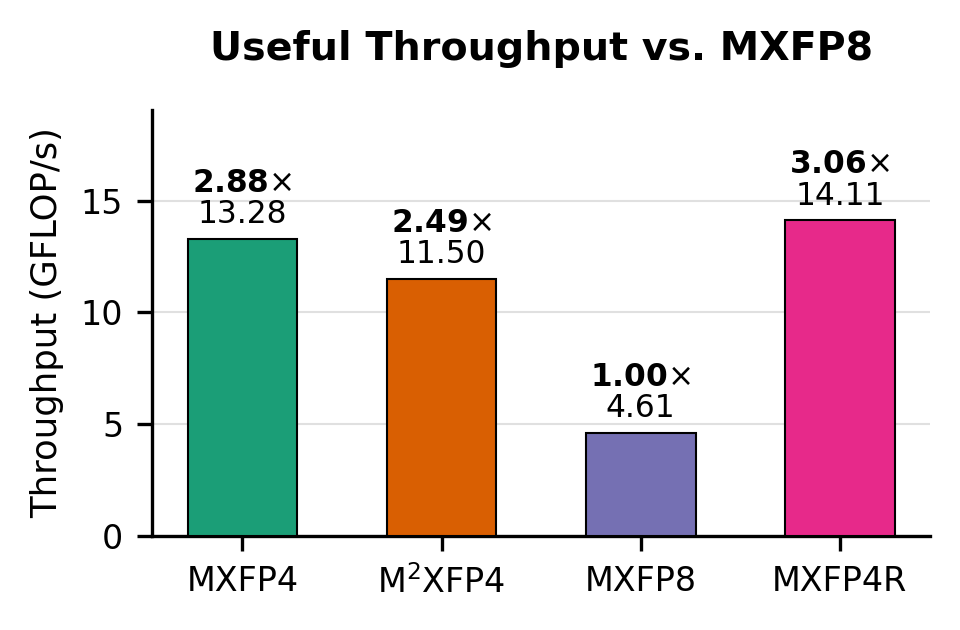
\includegraphics[width=\linewidth]{mxfp4r_throughput_comparison.png}
  \end{minipage}
\end{table*}
